\iffalse
\documentclass[journal,12pt,twocolumn]{IEEEtran}
\usepackage{cite}
\usepackage{amsmath,amssymb,amsfonts,amsthm}
\usepackage{graphicx}
\usepackage{textcomp}
\usepackage{xcolor}
\usepackage{enumitem}
\usepackage{mathtools}
\usepackage{gensymb}
\usepackage{comment}
\usepackage[breaklinks=true]{hyperref}
\usepackage{tkz-euclide}
\usepackage{circuitikz}
\usepackage{pgfplots}
\usepackage{gvv}
\begin{document}

\bibliographystyle{IEEEtran}
\vspace{3cm}

\title{GATE 2022-PH}
\author{EE23BTECH1205 - Avani Chouhan$^{*}$}
\maketitle
\bigskip

\renewcommand{\thefigure}{\theenumi}
\renewcommand{\thetable}{\theenumi}

\vspace{3cm}
\textbf{Question : 11} \\
For the Op-Amp circuit shown below, choose the correct output waveform corresponding to the input \( V_{\text{in}} = 1.5 \sin(20 \pi t) \) (in Volts). The saturation voltage for this circuit is \( V_{\text{sat}} = \pm 10 \) V.
\begin{figure}[ht]
\centering
    
\begin{circuitikz}
\tikzstyle{every node}=[font=\large]
\draw [, line width=0.7pt](11.5,9.75) node[op amp,scale=1] (opamp2) {}; \draw [, line width=0.7pt](opamp2.+) to[short] (10,9.25); \draw [, line width=0.7pt] (opamp2.-) to[short] (10,10.25); \draw [, line width=0.7pt](12.7,9.75) to[short](13,9.75);
\draw [](10,10.25) to[short] (10,10.5);
\draw [](10,11) to[short] (10,10.5);
\draw[] (10,11) to[short] (6.75,11);
\draw [, line width=0.9pt](6.75,11) to[sinusoidal voltage source, sources/symbol/rotate=auto,l={ \large $V_{in}$}] (6.75,8.5);
\draw [line width=0.9pt](6.75,8.5) to (6.75,8.25) node[ground]{};
\draw [, line width=0.9pt](10,4.75) to[resistor , i=$I_1$] (10,8.25);
\draw [, line width=0.9pt](10,8.25) to[resistor , i=$I_2$] (14.25,8.25);
\draw [, line width=0.9pt](12.75,9.75) to[short] (13.75,9.75);
\draw [, line width=0.9pt](10,8.25) to[short] (10,9.25);
\draw [, line width=0.9pt](13.75,9.75) to[short] (14.25,9.75);
\draw [, line width=0.9pt](14.25,9.75) to[short] (14.25,8.25);
\draw [line width=0.9pt](10,5) to (10,4.75) node[ground]{};
\node [font=\large] at (13,10) {$V_{out}$};
\node [font=\large] at (12.25,7.5) {$20k\Omega$};
\node [font=\large] at (9,6.75) {$2.2k\Omega$};
\end{circuitikz}


\end{figure}
\begin{enumerate}
  \item[(A)]
  \begin{figure}[ht!]
    \centering
    
\begin{circuitikz}
\tikzstyle{every node}=[font=\small]

\draw [](8.75,9.75) to[short] (8.75,13.25);
\draw[, line width=0.5pt] (8.75,10) to[short] (8.5,10);
\draw[, line width=0.5pt] (8.75,10.75) to[short] (8.5,10.75);
\draw[, line width=0.5pt] (8.75,11.5) to[short] (8.5,11.5);
\draw[, line width=0.5pt] (8.75,12.25) to[short] (8.5,12.25);
\draw[, line width=0.5pt] (8.75,13) to[short] (8.5,13);
\node [font=\small] at (11,9.5) {Time };
\node [font=\small] at (8.25,13) {10};
\node [font=\small] at (8.25,12.25) {5};
\node [font=\small] at (8.25,11.5) {0};
\draw[, line width=0.5pt] (12.5,9.75) to[short] (8.75,9.75);
\draw [, line width=0.5pt](8.75,13) to[short] (9,13);
\draw [, line width=0.5pt](9,13) to[short] (9,10);
\draw [, line width=0.5pt](9,10) to[short] (9.75,10);
\draw [, line width=0.5pt](9.75,10) to[short] (9.75,13);
\draw [, line width=0.5pt](9.75,13) to[short] (10.5,13);
\draw [, line width=0.5pt](10.5,13) to[short] (10.5,10);
\draw [, line width=0.5pt](10.5,10) to[short] (11.25,10);
\draw [, line width=0.5pt](11.25,10) to[short] (11.25,13);
\draw [, line width=0.5pt](11.25,13) to[short] (12,13);
\draw [, line width=0.5pt](12,13) to[short] (12,10);
\draw [, line width=0.5pt](12,10) to[short] (12.5,10);
\node [font=\small] at (8.25,10.75) {-5};
\node [font=\small] at (8.25,10) {-10};
\node [font=\small] at (7.75,11) {Vout(volts)};
\end{circuitikz}

\end{figure}
  \item[(B)]  
  \begin{figure}[ht]
    \centering
    
\begin{circuitikz}
\tikzstyle{every node}=[font=\small]

\draw [](8.75,9.75) to[short] (8.75,13.25);
\draw[, line width=0.5pt] (8.75,10) to[short] (8.5,10);
\draw[, line width=0.5pt] (8.75,10.75) to[short] (8.5,10.75);
\draw[, line width=0.5pt] (8.75,11.5) to[short] (8.5,11.5);
\draw[, line width=0.5pt] (8.75,12.25) to[short] (8.5,12.25);
\draw[, line width=0.5pt] (8.75,13) to[short] (8.5,13);
\node [font=\small] at (11,9.5) {Time };
\node [font=\small] at (8.25,13) {10};
\node [font=\small] at (8.25,12.25) {5};
\node [font=\small] at (8.25,11.5) {0};
\draw[, line width=0.5pt] (12.5,9.75) to[short] (8.75,9.75);
\draw [, line width=0.5pt](8.75,13) to[short] (12.5,13);
\node [font=\small] at (8.25,10.75) {-5};
\node [font=\small] at (8.25,10) {-10};
\node [font=\small] at (7.75,11) {Vout(volts)};
\end{circuitikz}

\end{figure}
  \item[(C)] 
  \begin{figure}[ht]
    \centering
    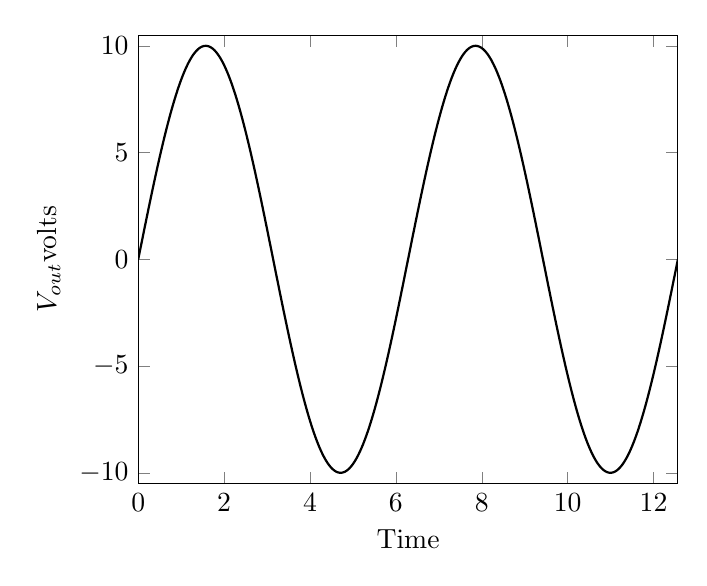
\begin{tikzpicture}
\begin{axis}[
    xlabel=Time,
    ylabel={$V_{out}$\brak{volts}},
    xmax=4*pi, xmin=0, 
    ymax=10.5, ymin=-10.5, % Adjust these values according to your data range
    ytick={-10,-5,0,5,10}, % Adjust these values according to your data range
    yticklabels={$-10$,$-5$,$0$,$5$,$10$}, % Adjust these values according to your data range
]
\addplot[domain=0:4*pi, samples=400, black, thick]{10*sin(deg(x))};
\end{axis}
\end{tikzpicture}

\end{figure}
  \item[(D)] 
   \begin{figure}[ht]
    \centering
    \begin{circuitikz}
\tikzstyle{every node}=[font=\small]
\draw [](8.75,9.75) to[short] (8.75,13.25);
\draw[, line width=0.5pt] (8.75,10) to[short] (8.5,10);
\draw[, line width=0.5pt] (8.75,10.75) to[short] (8.5,10.75);
\draw[, line width=0.5pt] (8.75,11.5) to[short] (8.5,11.5);
\draw[, line width=0.5pt] (8.75,12.25) to[short] (8.5,12.25);
\draw[, line width=0.5pt] (8.75,13) to[short] (8.5,13);
\node [font=\small] at (11,9.5) {Time };
\node [font=\small] at (8.25,13) {10};
\node [font=\small] at (8.25,12.25) {5};
\node [font=\small] at (8.25,11.5) {0};
\draw [, line width=0.5pt](8.75,11.5) to[short] (12.5,11.5);
\draw[, line width=0.5pt] (12.5,9.75) to[short] (8.75,9.75);
\node [font=\small] at (8.25,10.75) {-5};
\node [font=\small] at (8.25,10) {-10};
\node [font=\small] at (7.75,11.25) {$V_{out}$(volts)};
\end{circuitikz}

\end{figure}
\end{enumerate}

\hfill{(GATE PH 2022)}\\
\textbf{Solution:} \\
\fi
\begin{table}[htbp]
  \centering
  \begin{tabular}{|c|c|c|}
    \hline
    \textbf{Parameter} & \textbf{Value} & \textbf{description} \\ 
    \hline
    $Vin$ & $1.5 \sin(20\pi t)$ & input at inverting terminal \\
    \hline
    $V_{sat}$ & $\pm 10 \, \text{V}$ & saturation voltage\\
    \hline
    $V_{o}$ & $-$ & output voltage of the op-amp \\
    \hline
    $I_1$ & - & Current through $2.2k\Omega$  \\
    \hline
    $I_2$ & - & Current through $20k\Omega$  \\
    \hline
\end{tabular}


  \caption{Input Parameters}
\end{table}
\begin{align}
V_{in} &= 1.5 \sin(20\pi t)\\
V_{\text{sat}} &= \pm 10 \, \text{V}
\end{align}
Due to the virtual short voltage at the non-inverting terminal, which is\( V_{\text{in}} \) and $I_1 = I_2$,\\
\begin{align}
\frac{0 - V_{\text{in}}}{2.2 \, \text{k}\Omega} &= \frac{V_{\text{in}} - V_o}{20 \, \text{k}\Omega}\\
\frac{-20}{2.2} &= \frac{V_{\text{in}} - V_o}{V_{\text{in}}}\\
\frac{-20}{2.2} &= 1 - \frac{V_o}{V_{\text{in}}}\\
\frac{V_o}{V_{\text{in}}} &= 1 + \frac{20}{2.2}\\
V_o &\sim 10 V_{\text{in}}\\
V_o &= 10 \times 1.5 \sin(20\pi t)
\end{align}

Output amplitude is greater than $V_{\text{sat}}$, so the voltage saturates at $V_{\text{sat}}$.\\
Therefore, correct answer is (A).
%\end{document}
